\chapter{Research Methodology}\label{ch:research-methodology}
%\lipsum[2-8]
\initial{F}rom the literature there is a clear lack of results for localisation systems using the commercial Pozyx sensor network with drones in a household environment.
To address the aims and objectives stated in ~\ref{sec:aims_objs}, it is proposed that a lightweight onboard localisation be developed to check the feasibility of minimal hardware solution for an indoor drone.
This would entail connecting a Pozyx tag directly to an FCU and integrate it with the pose localisation system existing already.
To close the loop the pose information should be available in some format that can be used for autonomous control.
Furthermore, the system should be tested in a practical environment, to this end, the Pozyx anchor network was set up in a kitchen.
A kitchen represents one of the highest traffic areas in a household and it contains various materials that will make raw readings from a UWB system noisy and inaccurate.
As a kitchen will contain both dynamic and static obstacles multiple anchor configurations must be tested in order to find optimal anchor positions in this given environment.

\section{Anchor Configurations}\label{sec:anchor-configurations}
Noting work from ~\citet{di2019evaluation} and the setup procedures from ~\citet{pozyx2018pozyx} it is important to have at least 4 anchors setup in non-planar orientations for the best positioning results.
To determine a suitable anchor configuration in the given space a tag was placed at a fixed known point in a given reference frame and the mounted locations of the 4 anchors were varied on each wall of the kitchen in order to prevent planar configurations and ambiguity when the tag calculates its position.
Figure ~\ref{fig:layout} shows a simplified layout and toybox configuration of the tag and anchors.
Grey areas represent areas in the space that is impossible to traverse, red represents known obstacles that interfere and attenuate the UWB signal, blue represent anchors, green the tag, cream is partially obstructed and the rest of the area is fully traversable.
Before each run and data collection, the tag was manually configured with the location of each of the anchors in the reference frame of the kitchen and recorded for at least 5 seconds.
The tag was triggered to calculate the position repeatedly within the timeframe and the function call is blocking and takes $\approx70ms$ so data was recorded at a frequency of $\approx14.28Hz$.
With a tag position of (1480,2330,980)mm, the following statistics were calculated using Matlab.
In addition to the average error and standard deviation,  kurtosis and skew metrics were added to show the number of outliers and symmetry of the recorded data.
The error metrics are important to give an idea of how noisy the overall data is while kurtosis and skewness give an indication if the noise follows a uniform distribution which would be beneficial ideal for state estimators.
From table ~\ref{tb:config_stats} we can see that configuration 12 gives acceptable error metrics and reasonable skew and kurtosis making it the best out of the configurations tested.
To further support this Figure ~\ref{fig:config} shows several results obtained with several configurations and it can be seen that configuration 12 produced the best results with minimal noise and measurement outliers as well as it was centered around the ground truth position of the tag.

\begin{figure}[h!]
    \centering
    \includegraphics{mtd/Kitchen_layout}
    \caption{Bird's eye view of the test environment.}
    \label{fig:layout}
\end{figure}
\newpage

\begin{longtable}[h!]{| c | c |}
    \hline
    Config & Anchor positions (mm)$\left(\begin{array}{c}
   Anchor1(x,y,z),\\Anchor2(x,y,z),\\Anchor3(x,y,z),\\ Anchor4(x,y,z)
   \end{array}\right)$ \\
    \hline
    1 & $\left(\begin{array}{c}
   (0,0,1115),\\(3680, -405, 1550),\\(3655, 4080, 1906),\\(270, 4465, 2090)
   \end{array}\right)$\\
    \hline
    2 & $\left(\begin{array}{c}
   (0,665,1115),\\(2995, -405, 1889),\\(3655, 4080, 1906),\\(270, 4465, 2090)
   \end{array}\right)$\\
    \hline
    3 & $\left(\begin{array}{c}
   (0,665,1115),\\(2995, -405, 1889),\\(3655, 4080, 1906),\\(1526, 4559, 837)
   \end{array}\right)$\\
    \hline
    4 & $\left(\begin{array}{c}
   (0,665,1115),\\(2995, -405, 1889),\\(3655, 4080, 1906),\\(1070, 5170, 491)
   \end{array}\right)$\\
    \hline
    5 & $\left(\begin{array}{c}
   (0,665,1115),\\(2995, -405, 1889),\\(3960, 3368, 2304),\\(1070, 5170, 491)
   \end{array}\right)$\\
    \hline
    6 & $\left(\begin{array}{c}
   (0,665,1115),\\(2737, -410, 1913),\\(3655, 3598, 1668),\\(1187, 4760, 590)
   \end{array}\right)$\\
    \hline
    7 & $\left(\begin{array}{c}
   (0,665,1115),\\(2737, -410, 1913),\\(3655, 4529, 1777),\\(1187, 4760, 590)
   \end{array}\right)$\\
    \hline
    8 & $\left(\begin{array}{c}
   (0,645,1214),\\(2737, -410, 1913),\\(3651, 4120, 1853),\\(1066, 4760, 491)
   \end{array}\right)$\\
    \hline
    9 & $\left(\begin{array}{c}
   (0,645,1214),\\(2737, -410, 1913),\\(3970, 3063, 2320),\\(1066, 4760, 491)
   \end{array}\right)$\\
    \hline
    10 & $\left(\begin{array}{c}
   (0,645,1214),\\(2737, -410, 1913),\\(3651, 3550, 1810),\\(1066, 4760, 491)
   \end{array}\right)$\\
   \hline
    11 & $\left(\begin{array}{c}
   (0,645,1214),\\(2737, -410, 1913),\\(3651, 3550, 1810),\\(1591, 4450, 1775)
   \end{array}\right)$\\
    \hline
    \rowcolor{LightGreen}12 & $\left(\begin{array}{c}
   (0,645,1214),\\(2737, -410, 1913),\\(3651, 4120, 1853),\\(1591, 4450, 1775)
   \end{array}\right)$\\
    \hline
    \caption{Anchor locations for each Configuration}
    \label{tb:ach_loc}
\end{longtable}

%\begin{table}[h!]
   \begin{longtable}[h!]{| c | c | c | c | c |}
       \hline
       Config
       & Avg. Error & Std. Deviation$\left(\begin{array}{c}
       x,\\y,\\z
       \end{array}\right)$ & Kurtosis & Skewness\\
       \hline
       1 & 342.5906 & $\left(\begin{array}{c}
       183.1707,\\205.3426,\\972.6239
       \end{array}\right)$&$\left( \begin{array}{c}
       2.349,\\ 1.5967,\\ 1.415
       \end{array} \right)$&$\left( \begin{array}{c}
       -0.4083,\\ -0.3522,\\ 0.4551
       \end{array} \right)$\\
       \hline
              2 &  173.5938 & $\left(\begin{array}{c}
       43.2345,\\45.6897,\\133.8616\\
       \end{array}\right)$&$\left( \begin{array}{c}
       21.8923,\\ 10.1765,\\ 119.1344
       \end{array} \right)$&$\left( \begin{array}{c}
       -2.8672,\\ -0.3453,\\ 8.9025
       \end{array} \right)$\\
       \hline
              3 &  203.8502 & $\left(\begin{array}{c}
       128.4693,\\118.3216,\\209.1637
       \end{array}\right)$&$\left( \begin{array}{c}
       14.2955,\\ 11.2045,\\ 2.9124
       \end{array} \right)$&$\left( \begin{array}{c}
       -2.579,\\  -0.3920,\\ 0.4055
       \end{array} \right)$\\
       \hline
              4 &  85.8562 & $\left(\begin{array}{c}
       40.2197,\\40.6081,\\66.2120
       \end{array}\right)$&$\left( \begin{array}{c}
       6.7558,\\ 7.5180,\\ 3.4722
       \end{array} \right)$&$\left( \begin{array}{c}
       -0.4260,\\ -0.5344,\\ -0.1242
       \end{array} \right)$\\
       \hline
              5 &  64.8616 & $\left(\begin{array}{c}
       65.3883,\\53.8458,\\78.5751
       \end{array}\right)$&$\left( \begin{array}{c}
       13.3707,\\ 13.2178,\\ 11.0111
       \end{array} \right)$&$\left( \begin{array}{c}
       -0.6016,\\ 0.3745,\\ 0.0461
       \end{array} \right)$\\
       \hline
              6 &  189.933 & $\left(\begin{array}{c}
       40.8435,\\32.6482,\\58.5618
       \end{array}\right)$&$\left( \begin{array}{c}
       11.8957,\\ 11.8924,\\ 11.092
       \end{array} \right)$&$\left( \begin{array}{c}
       0.7516,\\ -0.0100,\\ -0.1322
       \end{array} \right)$\\
       \hline
              7 &  100.6929 & $\left(\begin{array}{c}
       75.8269,\\72.0940,\\41.9398
       \end{array}\right)$&$\left( \begin{array}{c}
       26.0285,\\ 17.4295,\\ 7.2328
       \end{array} \right)$&$\left( \begin{array}{c}
       -3.1681,\\ -0.8384,\\ -0.7151
       \end{array} \right)$\\
       \hline
              8 &  138.1276 & $\left(\begin{array}{c}
       26.2243,\\21.8750,\\70.6189
       \end{array}\right)$&$\left( \begin{array}{c}
       4.6048,\\ 52.2374,\\ 50.9467
       \end{array} \right)$&$\left( \begin{array}{c}
       -0.4858,\\ 5.0752,\\ 5.1757
       \end{array} \right)$\\
       \hline
              9 &  258.296 & $\left(\begin{array}{c}
       165.7105,\\95.081,\\475.0623
       \end{array}\right)$&$\left( \begin{array}{c}
       2.2833,\\ 1.7939,\\ 2.3406
       \end{array} \right)$&$\left( \begin{array}{c}
       -0.6982,\\ 0.2746,\\ 0.7517
       \end{array} \right)$\\
       \hline
              10 &  235.348 & $\left(\begin{array}{c}
       116.1306,\\89.9868,\\420.8322
       \end{array}\right)$&$\left( \begin{array}{c}
       3.6670,\\ 4.7058,\\ 3.8066
       \end{array} \right)$&$\left( \begin{array}{c}
       1.5079,\\ -1.7613,\\ -1.5615
       \end{array} \right)$\\
       \hline
              11 &  223.4468 & $\left(\begin{array}{c}
       120.9674,\\79.8602,\\409.8192
       \end{array}\right)$&$\left( \begin{array}{c}
       3.389,\\ 4.6663,\\ 3.1988
       \end{array} \right)$&$\left( \begin{array}{c}
       1.1099,\\ -1.5397,\\ -1.2038
       \end{array} \right)$\\
       \hline
              \rowcolor{LightGreen}12 &  111.8493 & $\left(\begin{array}{c}
       27.568,\\17.7124,\\64.4278
       \end{array}\right)$&$\left( \begin{array}{c}
       4.8522,\\ 7.4335,\\ 6.2489
       \end{array} \right)$&$\left( \begin{array}{c}
       -0.0239,\\ -0.8535,\\ 3.7132
       \end{array} \right)$\\
       \hline
       \caption{Statistics of the data recorded for each configuration.}
        \label{tb:config_stats}
   \end{longtable}
%\end{table}

    \begin{figure}[h!]
        \centering
        \begin{subfigure}[b]{0.49\textwidth}
            \includegraphics[width=\textwidth]{results/config1}
            \caption{Plot of Config 1}
        \end{subfigure}
        ~ %add desired spacing between images, e. g. ~, \quad, \qquad, \hfill etc.
          %(or a blank line to force the subfigure onto a new line)
        \begin{subfigure}[b]{0.49\textwidth}
            \includegraphics[width=\textwidth]{results/config2}
            \caption{Plot of Config 2}
        \end{subfigure}

        \begin{subfigure}[b]{0.49\textwidth}
            \includegraphics[width=\textwidth]{results/config3}
            \caption{Plot of Config 3}
        \end{subfigure}
        ~ %add desired spacing between images, e. g. ~, \quad, \qquad, \hfill etc.
          %(or a blank line to force the subfigure onto a new line)
        \begin{subfigure}[b]{0.49\textwidth}
            \includegraphics[width=\textwidth]{results/config4}
            \caption{Plot of Config 4}
        \end{subfigure}

        \begin{subfigure}[b]{0.49\textwidth}
            \includegraphics[width=\textwidth]{results/config5}
            \caption{Plot of Config 5}
        \end{subfigure}
        ~ %add desired spacing between images, e. g. ~, \quad, \qquad, \hfill etc.
          %(or a blank line to force the subfigure onto a new line)
        \begin{subfigure}[b]{0.49\textwidth}
            \includegraphics[width=\textwidth]{results/config6}
            \caption{Plot of Config 6}
        \end{subfigure}
        \caption{Sample plots of several anchor configurations.}
        \label{fig:config}
    \end{figure}

    \begin{figure}\ContinuedFloat
        \begin{subfigure}[b]{0.49\textwidth}
            \includegraphics[width=\textwidth]{results/config7}
            \caption{Plot of Config 7}
        \end{subfigure}
        ~ %add desired spacing between images, e. g. ~, \quad, \qquad, \hfill etc.
          %(or a blank line to force the subfigure onto a new line)
        \begin{subfigure}[b]{0.49\textwidth}
            \includegraphics[width=\textwidth]{results/config8}
            \caption{Plot of Config 8}
        \end{subfigure}

        \begin{subfigure}[b]{0.49\textwidth}
            \includegraphics[width=\textwidth]{results/config9}
            \caption{Plot of Config 9}
        \end{subfigure}
        ~ %add desired spacing between images, e. g. ~, \quad, \qquad, \hfill etc.
          %(or a blank line to force the subfigure onto a new line)
        \begin{subfigure}[b]{0.49\textwidth}
            \includegraphics[width=\textwidth]{results/config10}
            \caption{Plot of Config 10}
        \end{subfigure}

        \begin{subfigure}[b]{0.49\textwidth}
            \includegraphics[width=\textwidth]{results/config11}
            \caption{Plot of Config 11}
        \end{subfigure}
        ~ %add desired spacing between images, e. g. ~, \quad, \qquad, \hfill etc.
          %(or a blank line to force the subfigure onto a new line)
        \begin{subfigure}[b]{0.49\textwidth}
            \includegraphics[width=\textwidth]{results/config12}
            \caption{Plot of Config 12}
        \end{subfigure}
        \caption[]{Sample plots of several anchor configurations. (cont'd)}
    \end{figure}


\begin{figure}[h!]
    \centering
    \begin{subfigure}[b]{0.4\textwidth}
            \includegraphics[width=\textwidth]{mtd/anchor1}
            \caption{Anchor 1}
    \end{subfigure}
    \begin{subfigure}[b]{0.4\textwidth}
            \includegraphics[width=\textwidth]{mtd/anchor2}
            \caption{Anchor 2}
    \end{subfigure}

    \begin{subfigure}[b]{0.4\textwidth}
            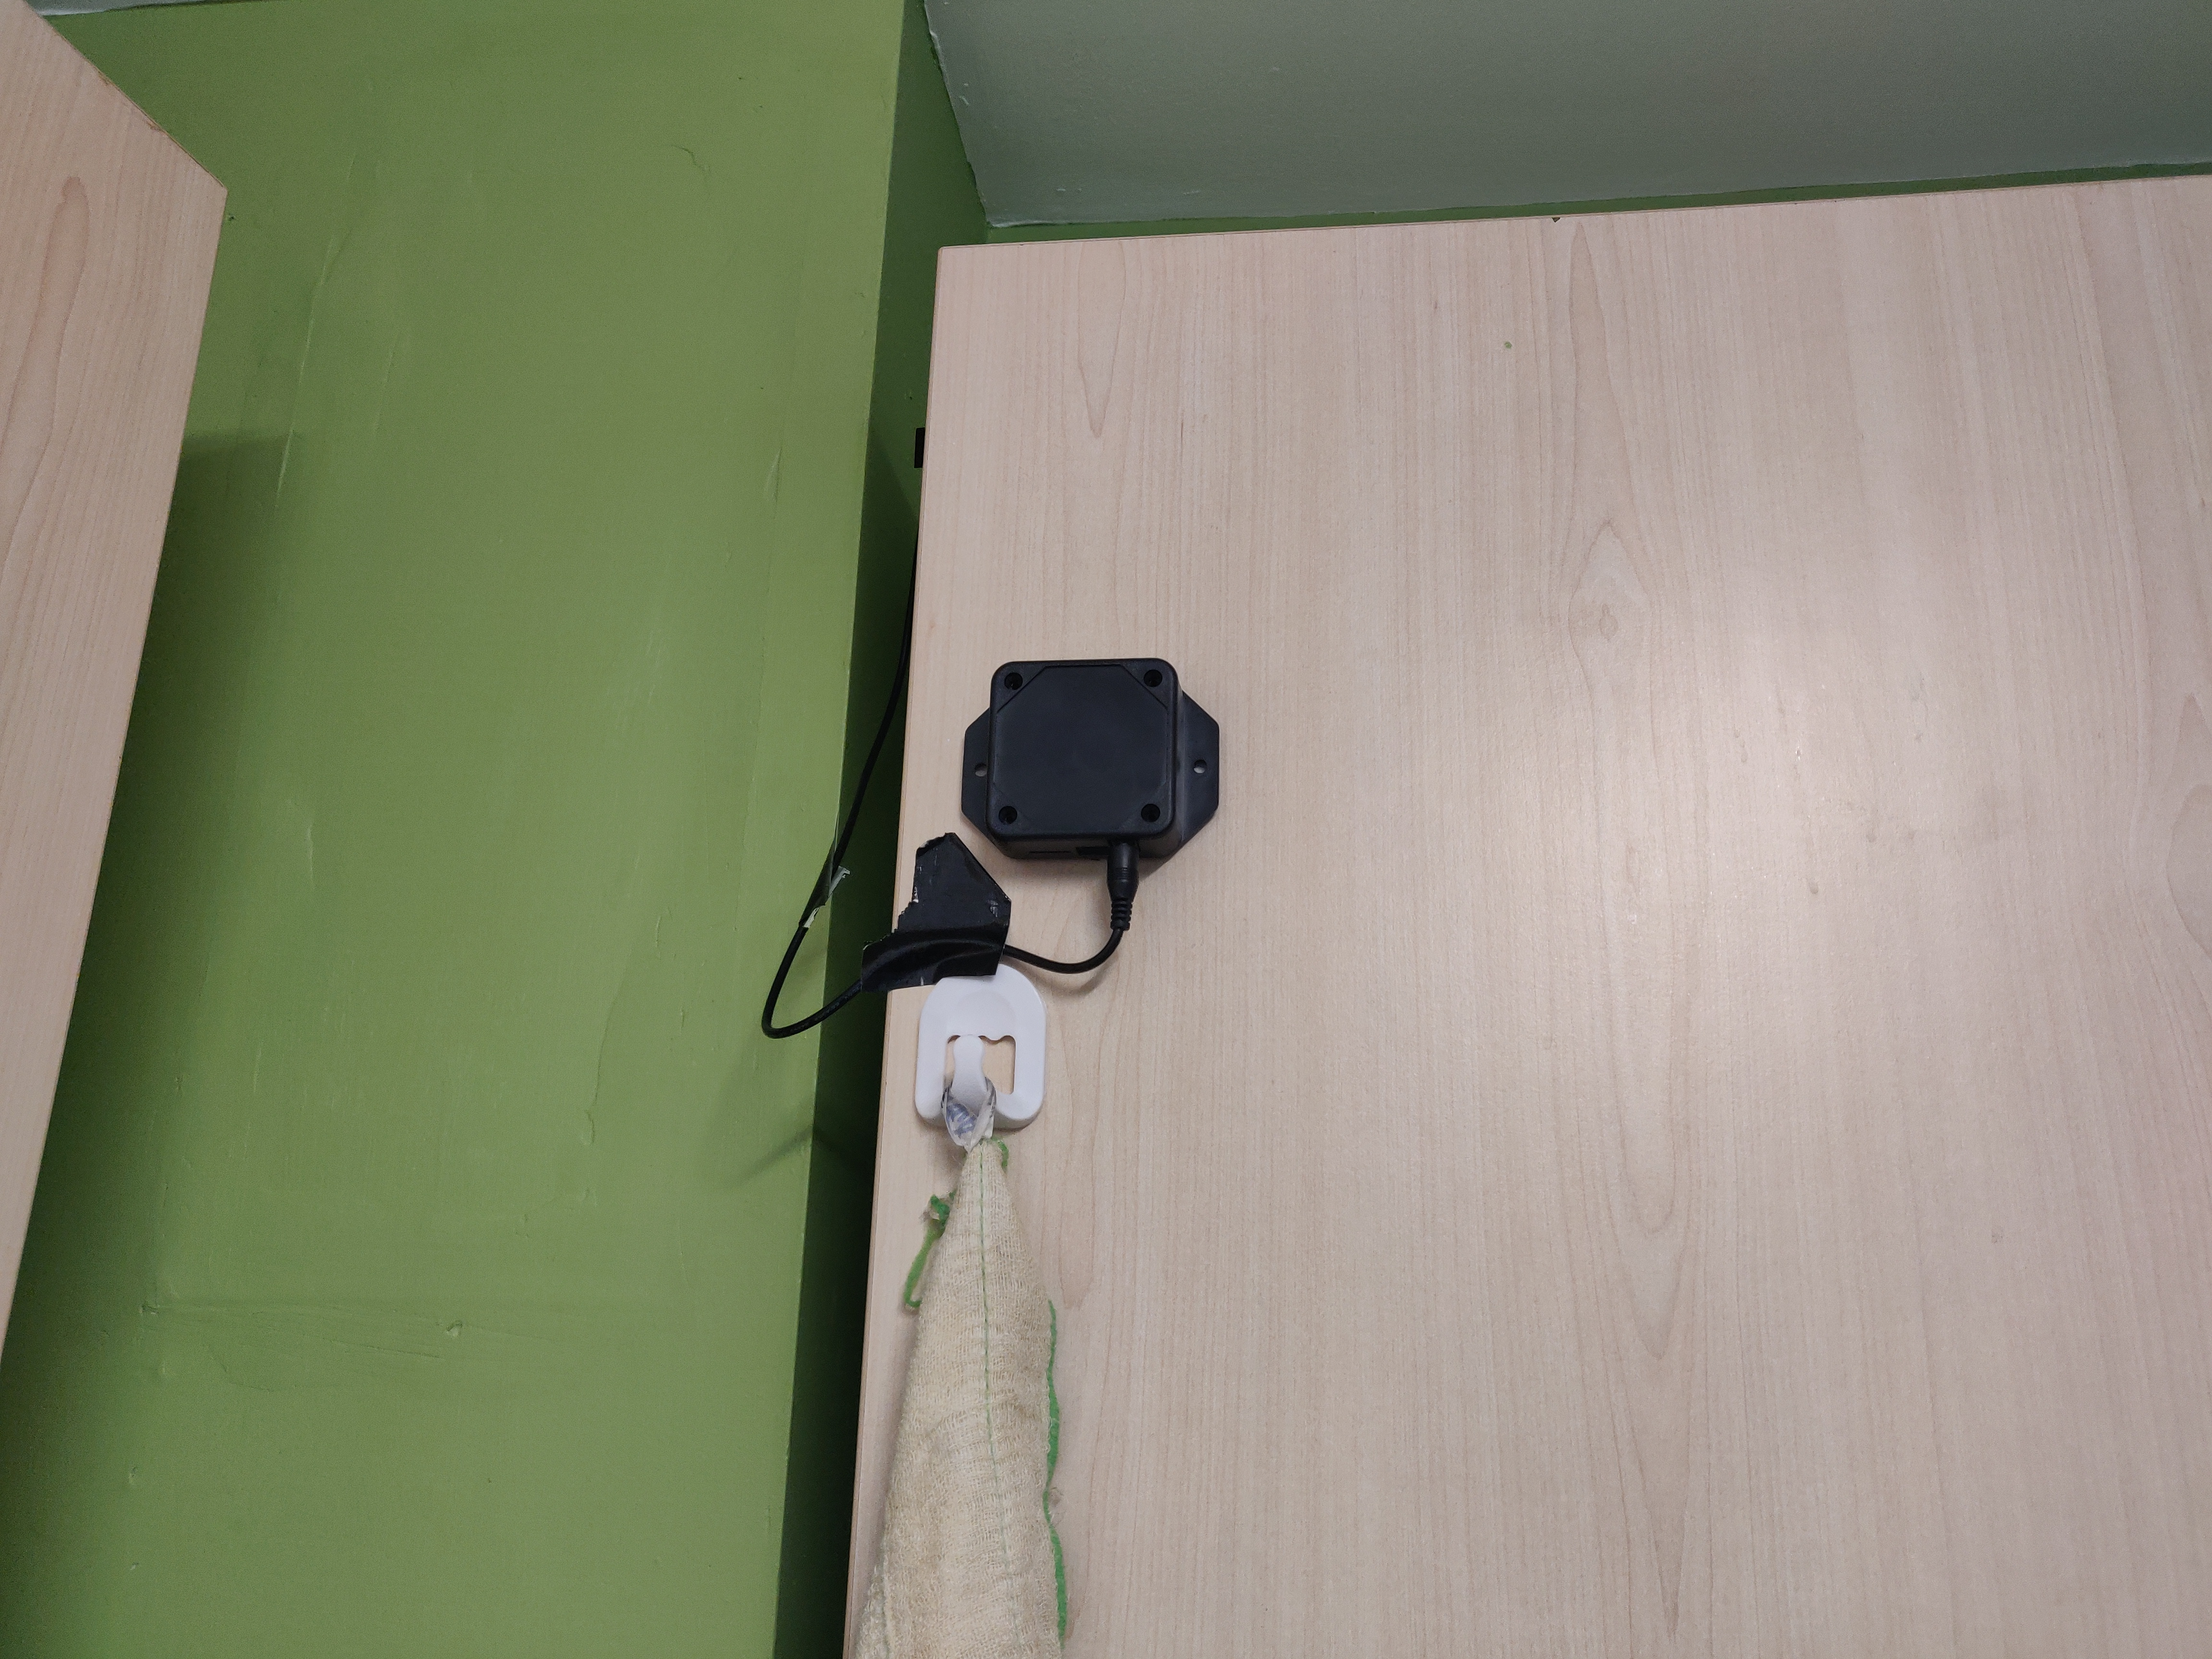
\includegraphics[width=\textwidth]{mtd/anchor3}
            \caption{Anchor 3}
    \end{subfigure}
    \begin{subfigure}[b]{0.4\textwidth}
            \includegraphics[width=\textwidth]{mtd/anchor4}
            \caption{Anchor 4}
    \end{subfigure}

    \begin{subfigure}[b]{0.7\textwidth}
            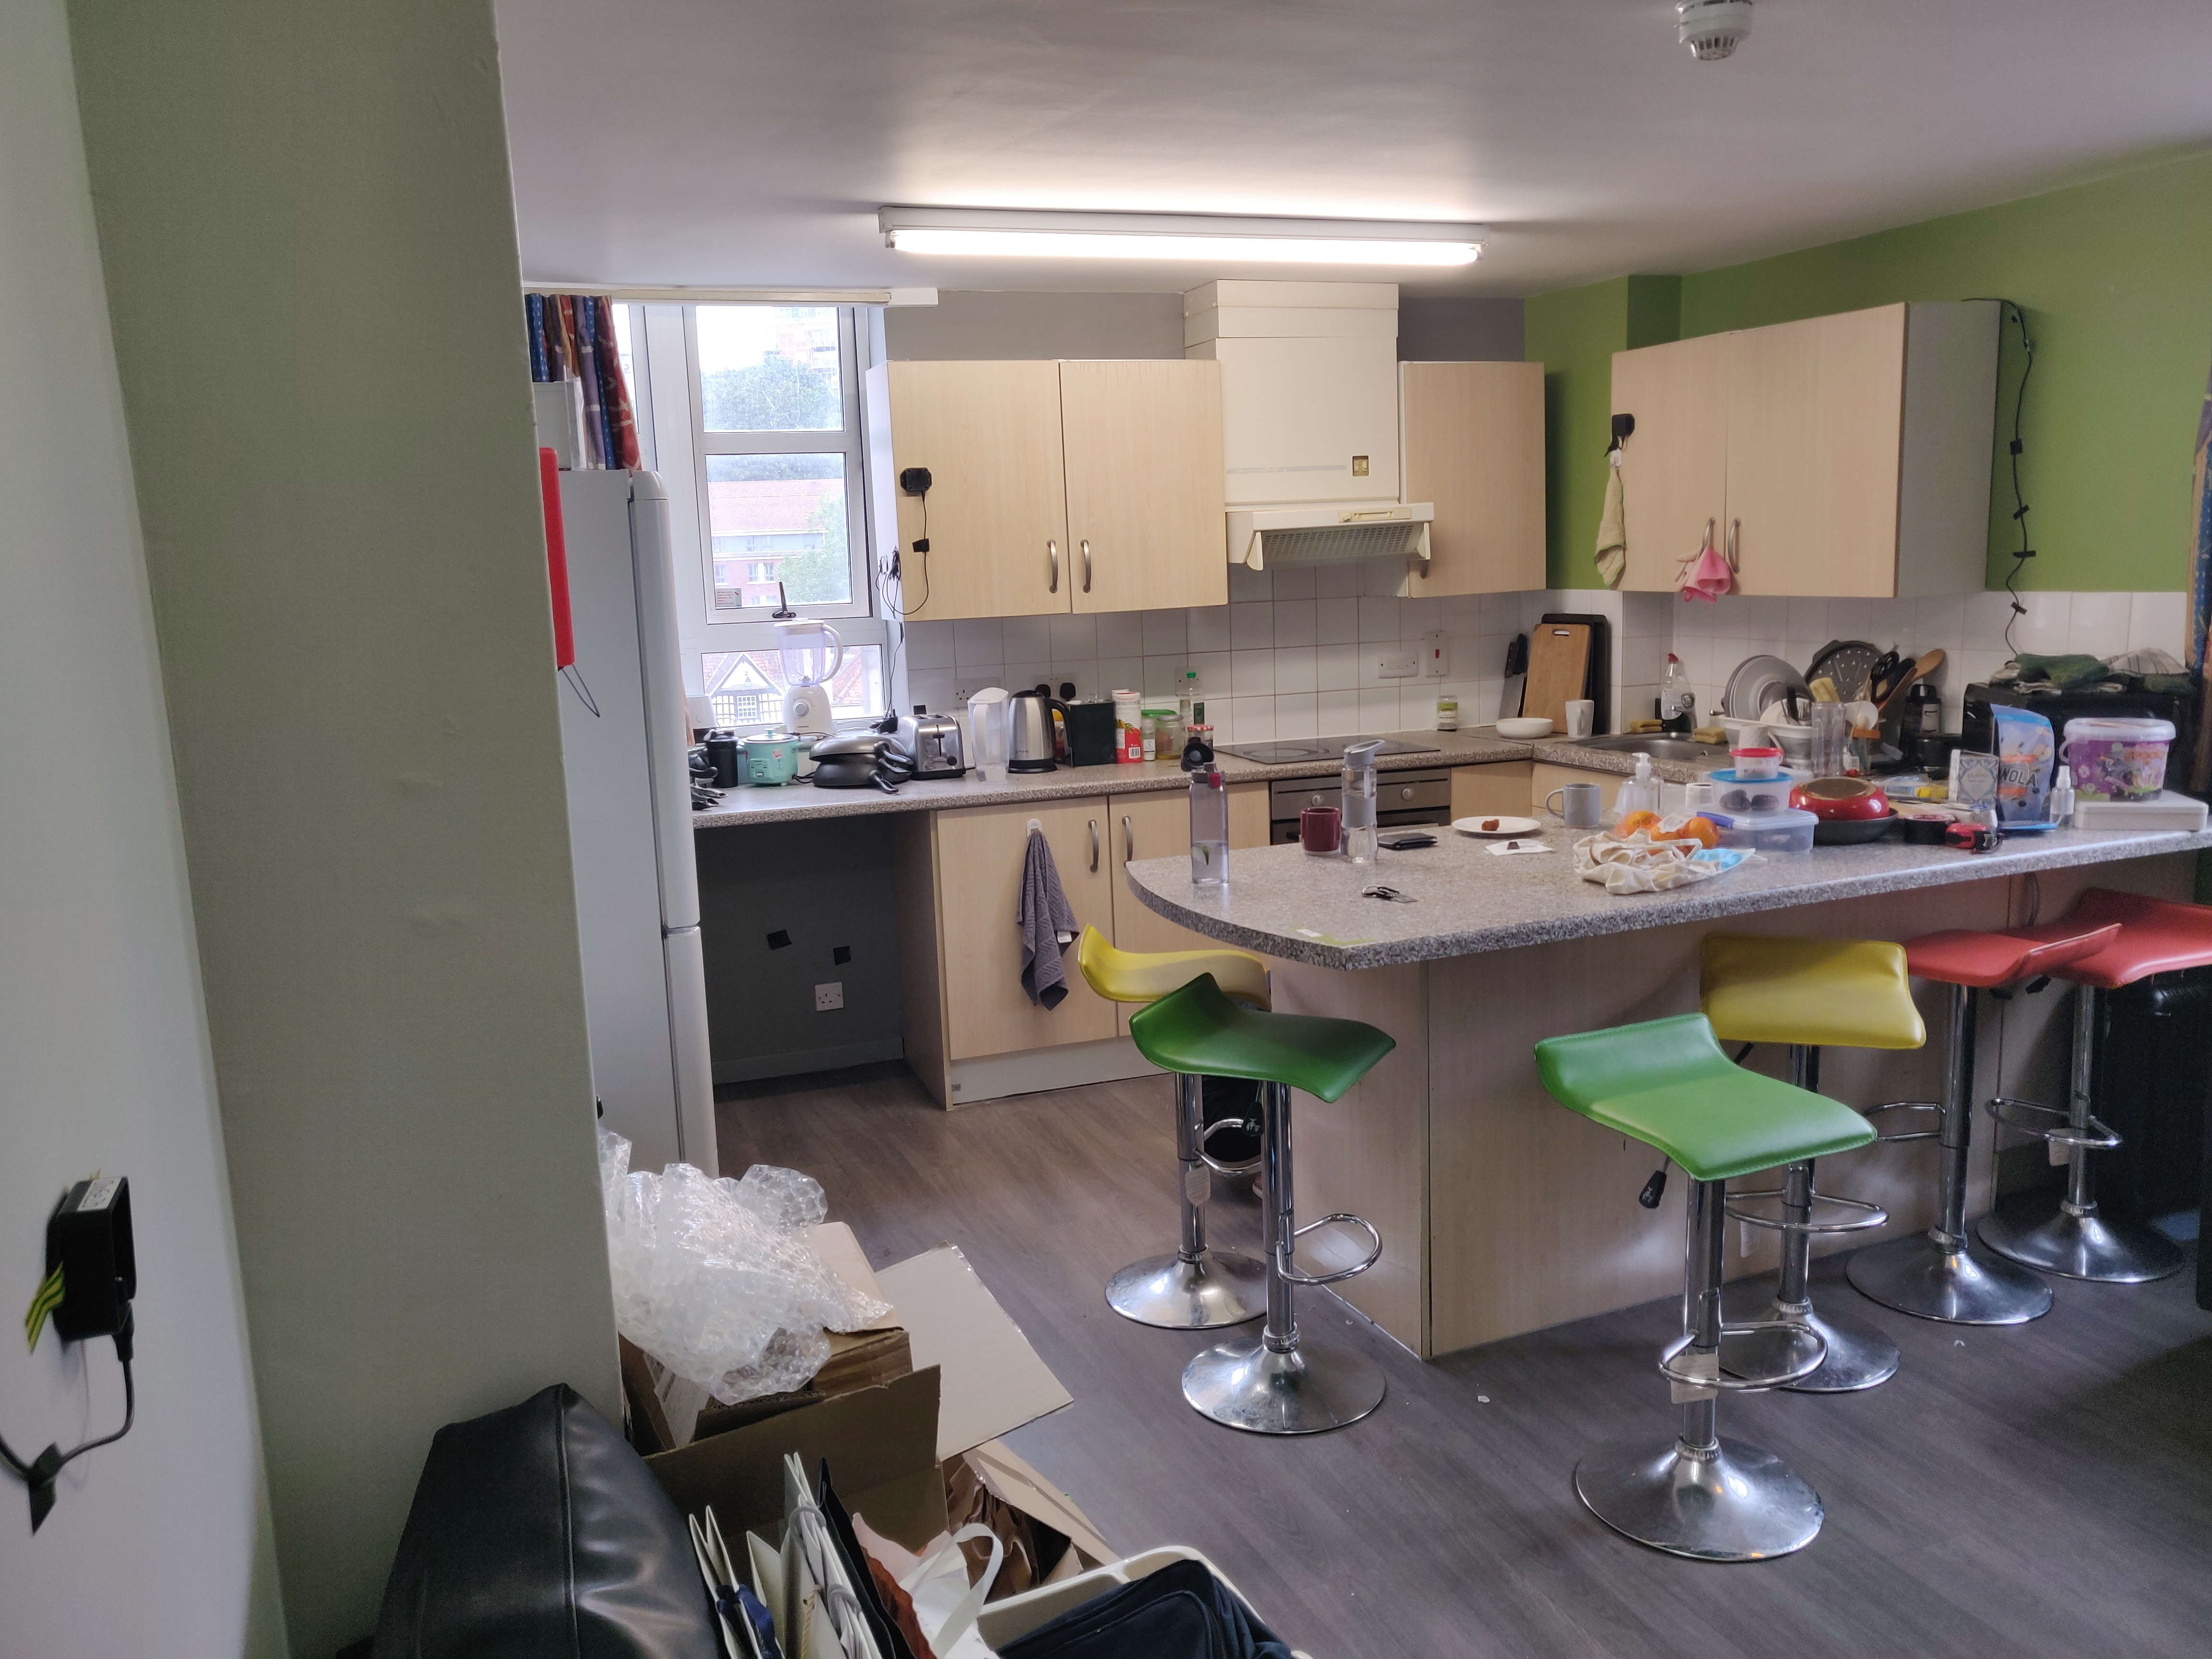
\includegraphics[width=\textwidth]{mtd/kitchen_full}
            \caption{Actual Kitchen Layout}
    \end{subfigure}
    \caption{Physical layout of the kitchen/Test Area}
    \label{fig:kitchen}
\end{figure}
\medskip
Figure: ~\ref{fig:kitchen} shows the physical locations of the Pozyx anchors with respect to obstacles in the environment.
Some things to note are:
\begin{itemize}
    \item The walls are made from concrete and drywall and there are no underlying materials that affected the performance of the anchors.
    \item The fridges have dimensions of $(600*600*1750)$mm.
    \item The corner of the island is located at $(1525,2106,918)$ and it has a dimension of $(2450*900*918)$mm.
    \item Above the island is considered traversable while beneath it will be considered to be impossible to traverse to simply future experiments.
\end{itemize}
%TODO: Insert the pics I took of the anchors here.
%Intro to the basic concept, highlight Pietra's paper and how I am using that to phrase and determine the best location
%Show pics, diagrams and initial table of results?

\subsection*{Summary}
The initial results allowed for a suitable configuration to be obtained but results were recorded in an ideal scenario.
Although these provide a good baseline for what to expect under good operational conditions, the parameters and limitations of the system would need to be tested before any form of optimisation
and improvement to position estimates can be done.
In the next Section: ~\ref{sec:op-params} we investigate this.

\newpage
\section{Operation Parameters}\label{sec:op-params}
\lipsum[2-4]
\newpage
\section{Technical Design}\label{sec:technical-design}
%\lipsum[2-8]
At the end of section:~\ref{sec:op-params} it was shown that using the raw position readings coming from the sensor is not feasbile in cases where NLOS is present.
Furthermore, the overall goal is for the position of an indoor UAV to be recovered with a fair amount of accuracy since this forms the basis of any autonomous behaviour and navigation.
As such it is desirable to use readings from multiple sensors but at the same time of reducing the overall physical footprint of the final system to keep it lightweight.
With that in mind it is proposed to directly integrate the POZYX sensor system with a motherboard unit that is capable of doing sensor fusion, UAV control and communicating with external systems.
In recent years FCU's have become versatile and robust and these requirements are easily met so in this section the technical parameters of the research will be discussed.

\subsection{Flight Controller Unit}\label{subsec:flight-controller-unit}
In order to prevent consuming too much time on dertermining a suitable flight system the Open-Source Hardware (OSH) community was consulted in order to find a suitable FCU for the research.
Survey work done by ~\citet{ebeid2018survey} present a qualitative analysis of several commercial hardware solutions.
Table:~\ref{tb:comparison} shows some of the major hardware considerations.
All of the units have the standard UART, PWM and I2C interfaces in addition to other onboard sensors and interfaces.
At the time of writing the Pixhawk series of FCU's are the most common and oldest systems.
They have all the standard interfaces as well as several sensors allowing making them a keen choice for developers and researchers in a plug and play platform.
Many in the series share the same intefaces with some of the smaller boards excluding some of the less popular interfaces.
As such, to allow for flexibility in the technical design one of the Pixhawk family was desirable for this research.
After deliberation and consulting the objectives and scope of this research it was determined that a basic Pixhawk would be satiable.
Figure:~\ref{fig:pix} shows the board chosen, it was shipped quickly and it contains everything necessary to meet the objectives of the project allowing for quick prototyping and proof of concepts.

\begin{table}[h!]
    \centering
    \begin{tabular}{|c | c | c | c | c|}
        \hline
        Platform & MCU & Sensors & Licenses & Interfaces\\
        \hline
        Pixhawk & STM32F427 & b, m & BSD & c, s, a, pp, sb, ds\\

        Pixhawk2 & STM32F427 & b, m & CC-BYSA-3.0 & c, s, a, pp, sb, ds\\

        PixRacer & STM32F427 & b' m & CC-BY 4.0 & c, pp, sb, ds \\

        Pixhawk 3 Pro & STM32F427 & b' m & CC-BY 4.0 & c, s, pp, sb, ds \\

        PX4 FMUv5 and v6 & STM32F427 & b' m & CC-BY 4.0 & c, s, a, pp, sb, ds \\

        CC3D & STM32F103 & None & GPLv3 & pp, ds, sb\\

        APM 2.8 & ATmega2560 & b & GPLv3 & pp, a\\

        Erle-Brain 3 & Raspberry Pi & b, m & CC BY-NC-SA &  a\\

        PXFmini & Raspberry Pi & b, m & CC BY-NC-SA & a\\
        \hline
    \end{tabular}
    \caption{Comparisons of various FCU's that are commercially available. Source: ~\citet{ebeid2018survey} Page: 2.}
    \label{tb:comparison}
    b: barometer, m: magnetometer, p: pitot tube sensor, c: CAN, s: SPI, a: ADC, pp:
PPM, sb: S.BUS, ds: DSM, da: DAC, x: XBEE, au: AUX, [d]: discontinued.
\end{table}

\begin{figure}[ht!]
    \centering
    \includegraphics[scale=0.7]{mtd/pixhawk}
    \caption{Radiolink Pixhawk used for the project}
    \label{fig:pix}
\end{figure}

Furthermore, since the chosen board is OSH it has several options of firmware that can be used which makes code and software developed on this system extendable to other boards given they are able to run the firmware.
\newpage

\subsection{Flight Firmware}\label{subsec:flight-firmware}
Now that a suitable FCU was chosen the next major step was determining a flight stack to run on the board.
The major firmware options for the Pixhawk are either Ardupilot or PX4 stack.
Both are well documented and have their advantages.
Both support a large array of vehicles but the major differences come from the licenses they are under.
Without delving into the technicalities of the licenses it is often summarised that PX4 is attractive to business owners who want to protect their property whilst Ardupilot pushes for changes to be put back into the main codebase.
Additionally, from a quick brief and use of each of the firmwares, Ardupilot is slightly more documented due to its general public license and a bit more user friendly in terms of compilation and flashing firmware thanks to its pythonic based wrapper for compilation and uploading.
Since both firmwares cover all the generic UAV types and there was no need for any niche systems Ardupilot was chosen as the primary codebase.
It is worth noting that there is a subsection of the Ardupilot codebase is dedicated to Beacon based positioning systems which a previous Pozyx implementation is coded ~\cite{ardupilotarduino}.

\subsection{Communication Interface (I2C vs Serial)}\label{subsec:communication-interfacei2c-vs-serial}
As mentioned in Chapter:~\ref{ch:literature-review} there is an implementation of using a Pozyx system in a GPS denied scenario ~\cite{ardupilotarduino}.
This shows that it is possible to get the positioning data into the Ardupilot codebase and have it interacting with the onboard sensor fusion systems.
A critique of this approach however is that it uses an additional Arduino Uno to pipe information from the Pozyx tag to the Pixhawk.
Given the availability of the standard interfaces onboard the Pixhawk and the scope and objectives of this research project it is feasible that the Uno can be stubbed out of this experiment and data can be integrated directly onto the Pixhawk.
This means the physical integration of the system can be summarised into the following steps:
\begin{itemize}
    \item Choose a suitable interface.
    \item Place the code within a suitable section of the codebase.
    \item Utilise the parent class of the section of the Ardupilot to integrate the sensor.
    \item After testing the base functionality, integrate the new library within the background scheduler so it can run and feed measurements in the background to the copter main code.
\end{itemize}

An Arduino ~\cite{pozarduino} and python library was originally designed by the Pozyx developers so it provided an algorithmic starting point for the functionality of the library being designed.
The Arduino library is based around the I2C protocol whilst the python module uses the serial interface.
As noted by the developers the python module is a port of the Arduino library and there is no plans to maintain the code and address bug fixes, as such the Arduino library was studied fo to build the new AP\_Bacon extension.
Furthermore, the I2C interface was designed onboard an embedded system so much of the flow can be ported effectively to the Pixhawk.
Lastly, the previous implementation uses the UART/serial interface so that avenue has already been explored so in the intrest of quick prototyping the I2C interface was chosen.
A positive note is that the existence of the prebuilt system allows data and experiments to be collected in lieu of development of this library since the information being provided is the same data generated by the Pozyx tag.
The design of this library proves that the sensor data can be integrated directly whilst the pre-built systems, which are stable, can be used for data collection and experiments.
%
%\begin{figure}[h!]
%    \centering
%    \includegraphics[scale=0.5]{}

%\end{figure}

\begin{figure}[ht!]
    \centering
    \includegraphics[width=\textwidth]{mtd/pozyx_uno}
    \caption{Non-GPS loiter solution provided by Ardupilot. Soruce:\url{https://ardupilot.org/copter/docs/common-pozyx.html}}
    %    \label{fig:pix}
\end{figure}

\begin{figure}[ht!]
    \centering
    \includegraphics[scale=0.6]{mtd/i2c_ifc}
    \caption{Proposed wiring of the I2C interface being developed}
\end{figure}

\begin{figure}[ht!]
    \centering
    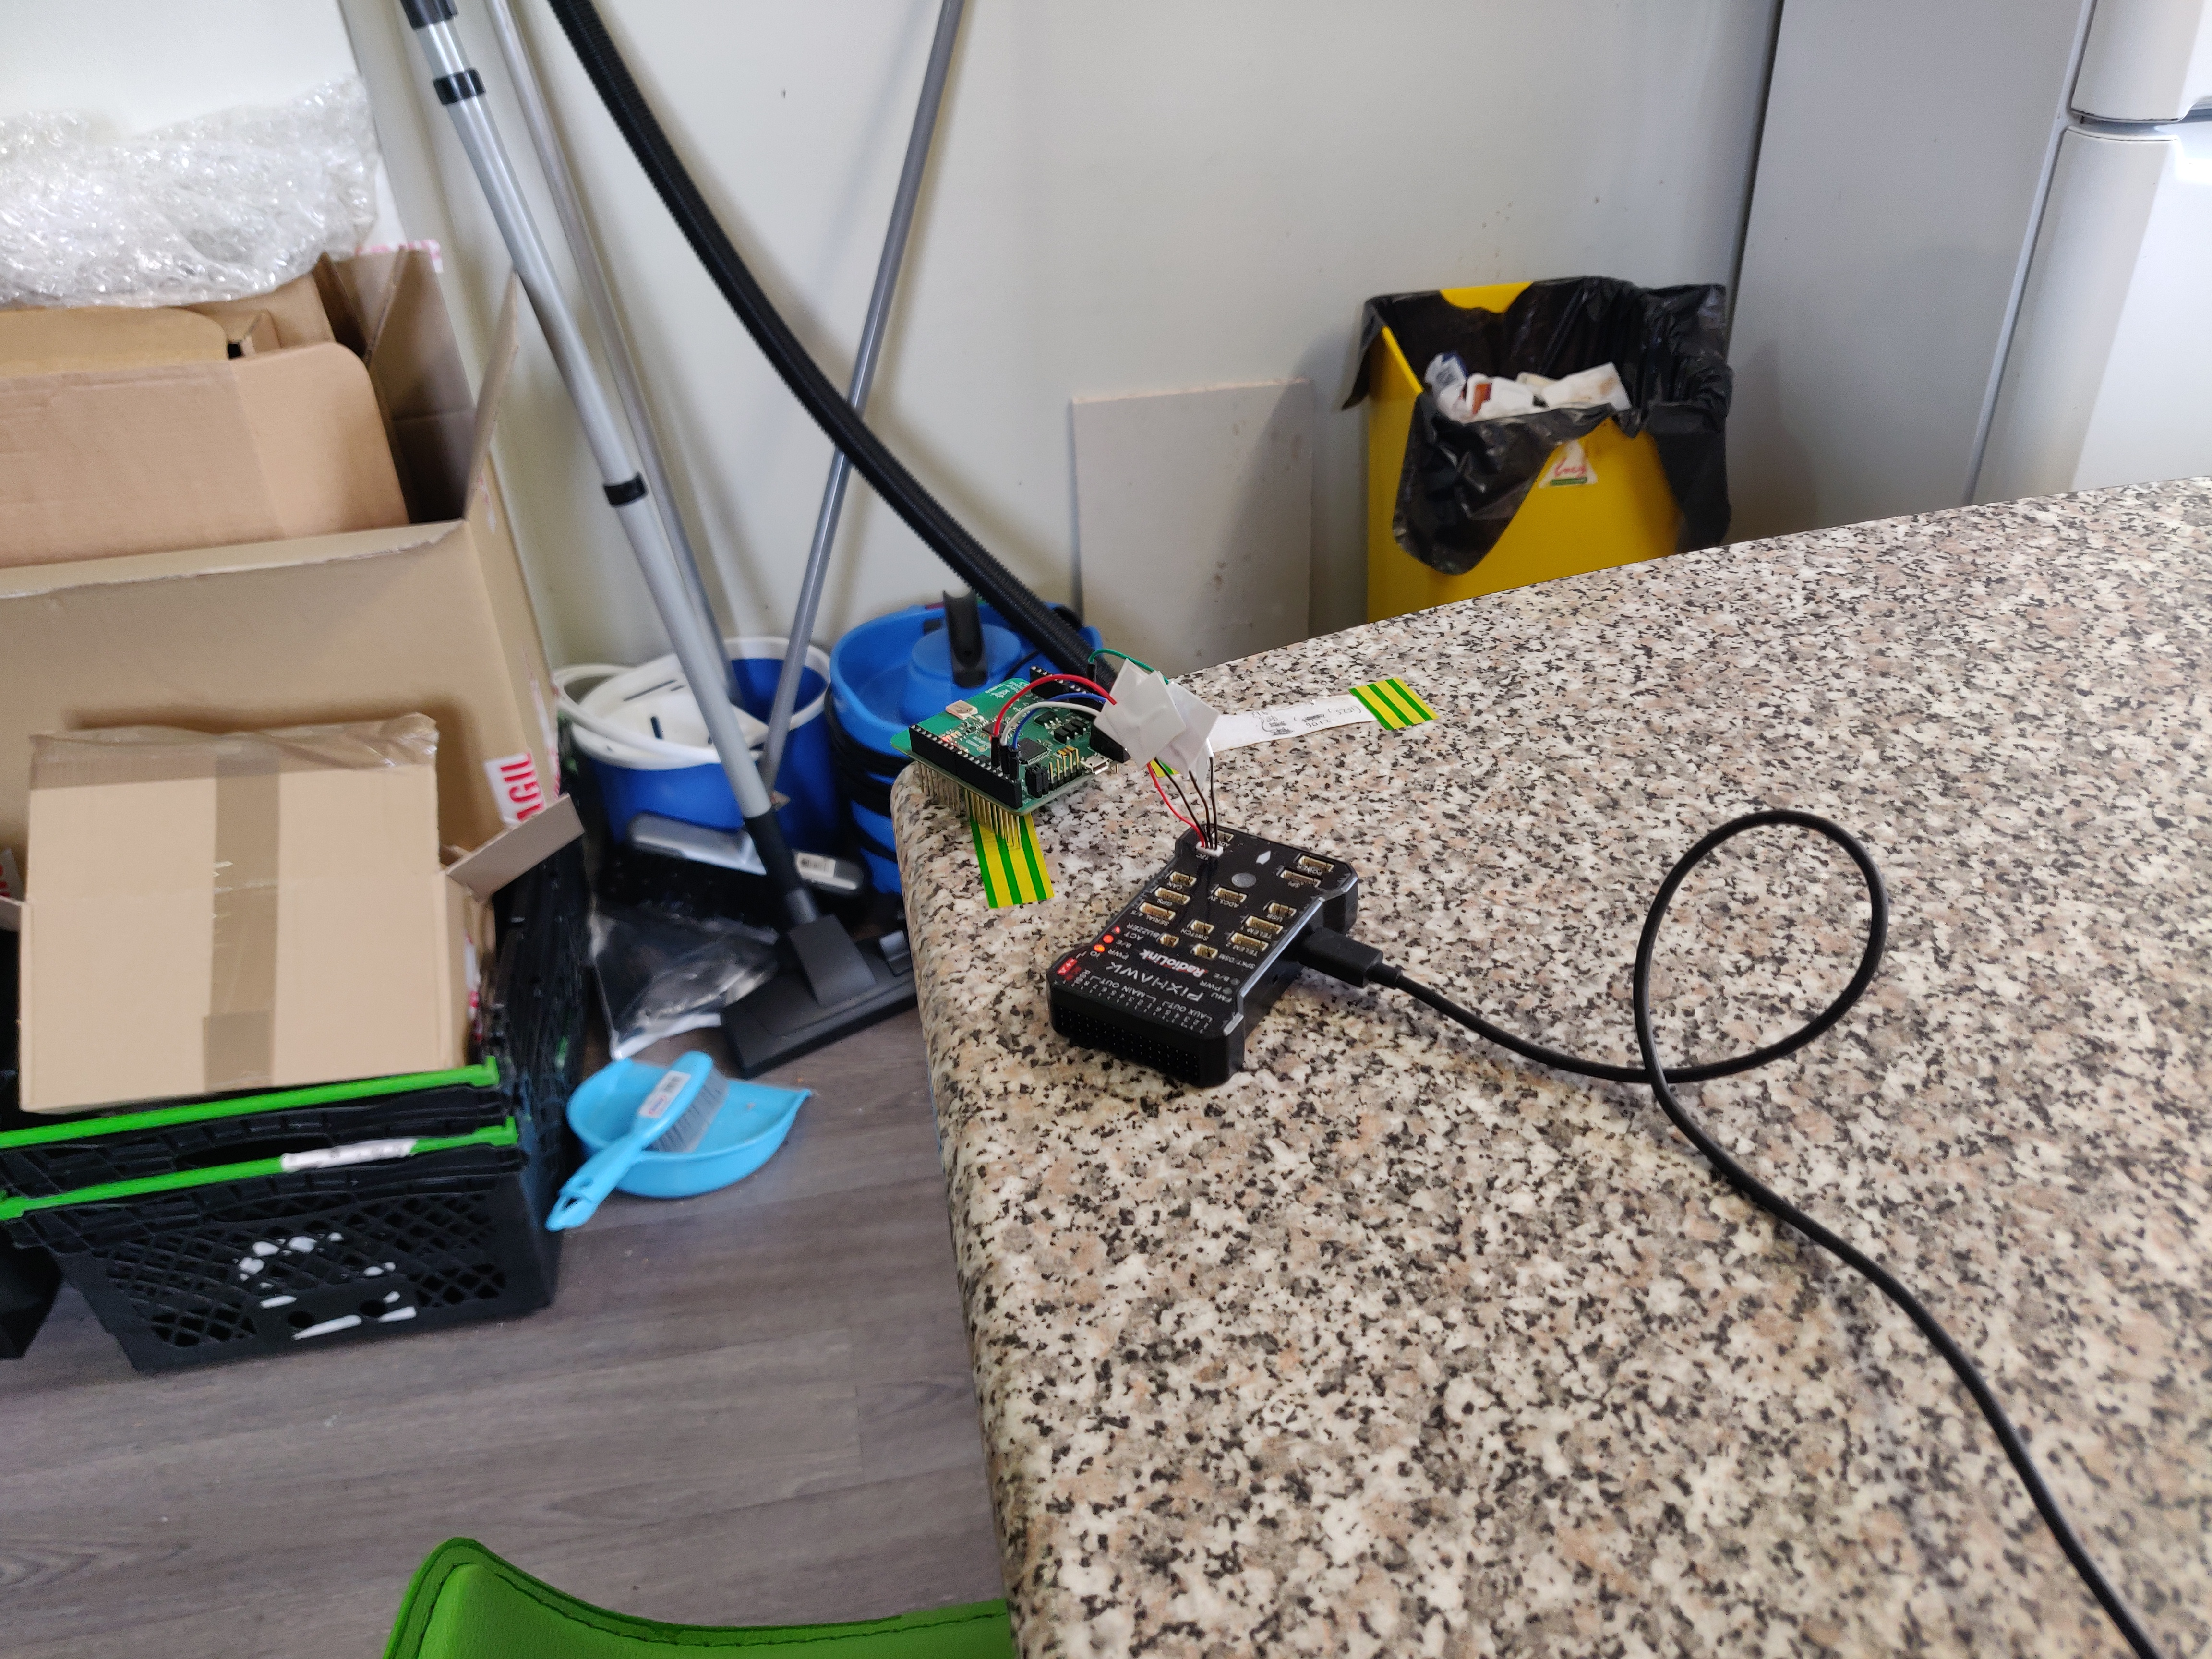
\includegraphics[width=\textwidth]{mtd/wip}
    \caption{System being unit tested in the environment.}
\end{figure}
\newpage
\subsection{Sensor Fusion: EKF on Ardupilot}\label{subsec:sensor-fusion}
\lipsum[2-6]